\documentclass[a4paper,11pt,exos]{nsi} % COMPILE WITH DRAFT
\usepackage{pifont}
\usepackage{fontawesome5}
\usepackage{hyperref}



\begin{document}
\classe{\terminale Comp}
\titre{Exercices - Intégration}
\maketitle

\tabularstyled[UGLiBlue]
\begin{tabular}{p{16.5cm}}
    \rowcolor{UGLiBlue}
    \ths Capacités attendues : \\

    \ding{111} Estimer graphiquement ou encadrer une intégrale, une valeur moyenne.   \\
    \ding{111} Calculer une intégrale, une valeur moyenne \\
    \ding{111} Calculer l’aire sous une courbe ou entre deux courbes.\\
    \ding{111} Interpréter une intégrale, une valeur moyenne dans un contexte issu d’une autre discipline.\\
\end{tabular}


\vspace*{.5cm}

\subsection*{Intégrale comme aire sous une courbe}

\dleft{10.3cm}{
    \exo{}
    Sur le graphique ci-contre sont données la droite représentant une fonction $f$ ainsi qu'une surface colorée.\\
    Déterminer par lecture graphique la valeur de l'intégrale $\displaystyle \int_{-3}^1 f(x) \, dx$.
}
{
    \def\xmin{-4} \def\ymin{-1}\def\xmax{2}\def\ymax{3}
    \def\F{2}
    \begin{tikzpicture}[scale=.95]
    \draw[fill=white] (\xmin,\ymin) rectangle (\xmax,\ymax);
        \draw[fill = UGLiOrange!30](-3,0) rectangle (1,2);
        \repereal{\xmin}{\ymin}{\xmax}{\ymax}
        \clip (\xmin,\ymin) rectangle (\xmax,\ymax);
        \draw[UGLiRed,domain=-3:1,smooth,variable=\x,thick] plot ({\x},{\F});
    \end{tikzpicture}
}

\vspace*{.5cm}

\dleft{10cm}{
    \exo{}
    Calculer la valeur de l'intégrale $\displaystyle \int_{0}^4 (-x+4) \, dx$.
}
{
    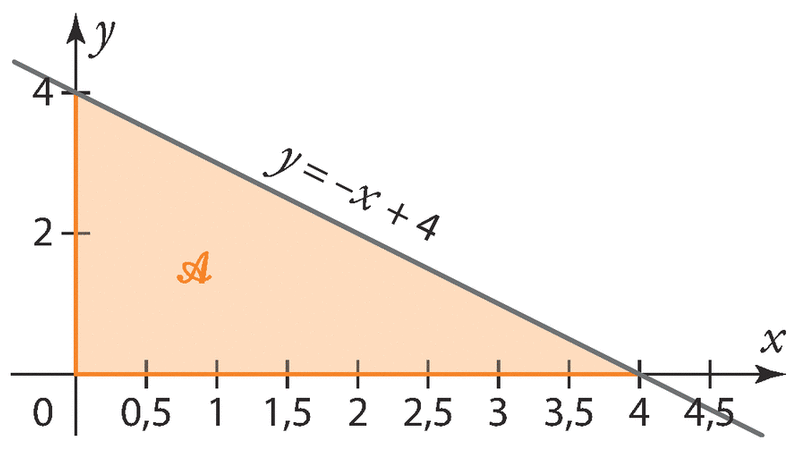
\includegraphics[width=6cm]{Sesamath30p152.png}
}

\vspace*{.5cm}

\dleft{10cm}{
	\exo{}
	Sur le graphique ci-contre sont représentées la courbe représentative d'une fonction $f$ définie sur $\fif{-2}{4}$ ainsi qu'une surface colorée.
	\begin{enumerate}
		\item Déterminer par lecture graphique l'expression de $f(x)$.
		\item Déterminer la valeur de l'intégrale $\displaystyle \int_{-2}^{2} f(x) \, dx$.
	\end{enumerate}
}
{
	\def\xmin{-3} \def\ymin{-1}\def\xmax{4}\def\ymax{5}
    \def\F{.5*\x+2}
    \begin{tikzpicture}[scale=.85]
    \draw[fill=white] (\xmin,\ymin) rectangle (\xmax,\ymax);
		\fill[UGLiOrange!30] 	(2,0)-- (-2,0) --
	plot[thick,domain=-2:2,smooth,variable=\x] ({\x},{\F})  --cycle;
        %\draw[fill = UGLiOrange!30](-3,0) rectangle (1,2);
        \repereal{\xmin}{\ymin}{\xmax}{\ymax}
        \clip (\xmin,\ymin) rectangle (\xmax,\ymax);
        \draw[UGLiRed,domain=-2:4,smooth,variable=\x,thick] plot ({\x},{\F});
    \end{tikzpicture}
}

\exo{}
Calculer chaque intégrale :
\begin{multicols}{5}
	\begin{enumerate}
		\item $\displaystyle \int_{0}^{2} 3 \, dx$
		\item $\displaystyle \int_{-1}^{4} 2 \, dx$
		\item $\displaystyle \int_{0}^{1} x \, dx$
		\item $\displaystyle \int_{0}^{5} (t+1) \, dt$
		\item $\displaystyle \int_{-1}^{1} (1-u) \, du$
	\end{enumerate}
\end{multicols}

\subsection*{Estimer une intégrale par la méthode des rectangles}

\begin{minipage}{10cm}
	\exo{}
	Voici la courbe représentative d'une fonction $f$ dans un repère orthonormal $\repaff$.\\
	On note $$\displaystyle I=\int_{-1}^{2}f(x)\text{d}x$$
	Encadrer $I$ par 2 entiers.
	
\end{minipage}\hspace*{.5cm}
\begin{minipage}{6.5cm}
			\def\xmin{-2}	\def\xmax{4}	\def\ymin{-1}	\def\ymax{5}
			\def\F{-(\x+1)*(\x-3)}
			\begin{tikzpicture}
				\repereal{\xmin}{\ymin}{\xmax}{\ymax}
				\clip	(\xmin,\ymin) rectangle (\xmax,\ymax);
				\fill[pattern =north east lines, pattern color = blue] 	(-1,0) --
				plot[thick,domain=-1:2,smooth,variable=\x] ({\x},{\F}) --
				(2,3)-- (2,0) --cycle;
				\draw[thick,domain=\xmin:\xmax,smooth,variable=\x]  plot ({\x},{\F});
			\end{tikzpicture}
		\end{minipage}
		
\vspace*{.5cm}
	
	
\begin{minipage}{6.5cm}
	\def\xmin{-2}\def\xmax{4}\def\ymin{-1}\def\ymax{6}
	\def\F{5+(\x+1)*(\x-3)}
	\begin{tikzpicture}
	\reperea{\xmin}{\ymin}{\xmax}{\ymax}
	\clip	(\xmin,\ymin) rectangle (\xmax,\ymax);
	\fill[pattern =north east lines, pattern color = blue] 	(0,0)-- (0,2) --
	plot[thick,domain=-0:3,smooth,variable=\x] ({\x},{\F}) --(3,5)-- (3,0) --cycle;
	\draw[thick,domain=\xmin:\xmax,smooth,variable=\x]  plot ({\x},{\F});
	\end{tikzpicture}
\end{minipage}
\begin{minipage}{10cm}
	\exo{}
	Voici la courbe représentative d'une fonction $g$ dans un repère orthonormal $\repaff$.\\
On note $$\displaystyle J=\int_{0}^{3}g(x)\text{d}x$$
\begin{enumerate}
	\item 	Encadrer $J$ par 2 entiers.
	\item 	Encadrer $J$ par 2 multiples de $0,25$ (compter les petits carreaux).
\end{enumerate}
\end{minipage}

\vspace*{1cm}

\dleft{10cm}{
	\exo{}
	La fonction $f$ définie sur $\fio{0}{+\infty}$ par $f(x)=\sqrt{x}$ est représentée dans le repère ci-contre.\\
	Utiliser les rectangles représentés pour estimer la valeur de l'intégrale $\displaystyle \int_{0}^{4}f(x) \, dx$.
}
{
	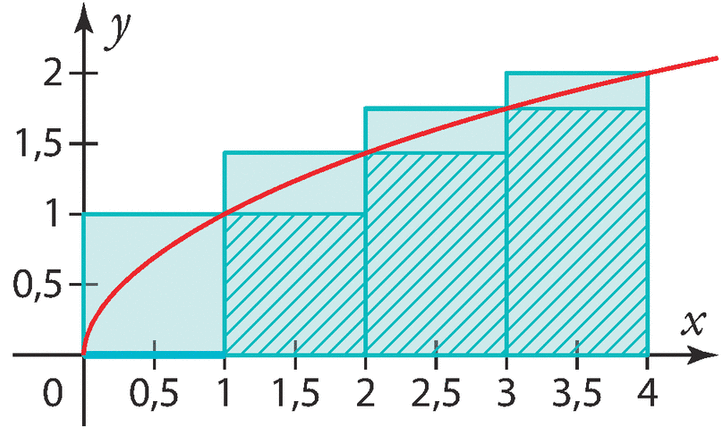
\includegraphics[width=6cm]{Sesamath35p152.png}
}

\vspace*{.5cm}

\dleft{10cm}{
	\exo{}
	$f$ est la fonction définie sur l'intervalle $\fif{0}{1}$ par $f(x)=e^x$.
	\begin{enumerate}
		\item Utiliser les rectangles de même largeur largeur représentés ci-contre pour déterminer un encadrement de l'intégrale $\displaystyle I=\int_{0}^{1} e^x \, dx$.
		\item En quel nombre $n$ d'intervalles de même longueur doit-on subdiviser $\fif{0}{1}$ pour obtenir un encadrement de $I$ d'amplitude $0,1$ ?
	\end{enumerate}
}
{
	\def\xmin{-.25} \def\ymin{-.5}\def\xmax{1.25}\def\ymax{3}
	\def\f{exp(\x)}
	\begin{tikzpicture}[xscale=4, yscale=1.5]
        \draw[thick, ->] (\xmin,0) -- (\xmax,0);
        \draw [thick, ->] (0,\ymin) -- (0,\ymax);
        \clip (\xmin,\ymin) rectangle (\xmax,\ymax);
        \draw[fill=UGLiBlue!30] (0,0) rectangle (.25,1.28);
		\draw[fill=UGLiBlue!30] (.25,0) rectangle (.5,1.65);
		\draw[fill=UGLiBlue!30] (.5,0) rectangle (.75,2.12);
		\draw[fill=UGLiBlue!30] (.75,0) rectangle (1,2.72);
		\fill[pattern =north east lines, pattern color = UGLiOrange] 	(0,0)-- (0,1) node[left]{$1$} -- (.25,1) -- (.25,0) --cycle;
		\fill[pattern =north east lines, pattern color = UGLiOrange] 	(.25,0) -- (.25,1.28) -- (.5,1.28) -- (.5,0) --cycle;
		\fill[pattern =north east lines, pattern color = UGLiOrange] 	(.5,0)node[below]{$0,5$}-- (.5,1.65) -- (.75,1.65) -- (.75,0) --cycle;
		\fill[pattern =north east lines, pattern color = UGLiOrange] 	(.75,0)-- (.75,2.12) -- (1,2.12) -- (1,0)node[below]{$0,1$}--cycle;
		\draw[UGLiRed,thick,domain=0:1,smooth,variable=\x] plot ({\x},{\f});
		\draw[dashed] (0,2.72) node[left] {$e$} -- (.75,2.72);
		\draw (-.02,2) -- (.02,2) ;
		\draw (0,2) node[left] {$2$};
		\draw[dashed] (0,1) -- (.25,1);
		\draw[dashed] (.25,1.28) -- (.5,1.28);
		\draw[dashed] (.5,1.65) -- (.75,1.65);
		\draw[dashed] (.75,2.12) -- (1,2.12);
	\end{tikzpicture}
}
\end{document}
